\chapter{Compare the domains}

I used \href{http://www.bioinformatics.nl/cgi-bin/emboss/dotmatcher}{\emph{EMBOSS} \textbf{dotmatcher}}, with the following parameters:

\begin{itemize}
\item window size: 100
\item threshold: 30.00
\end{itemize}

I chose the windows size to be that large, because I wanted to see if the whole sequence could be fitted in the window, how this algorithm would recognize the domains. However, if the \texttt{threshold} was too low, then the plot became too noisy -- these considerations led to the results, which are shown on Figure \ref{dotplot}


\begin{figure}
\centering
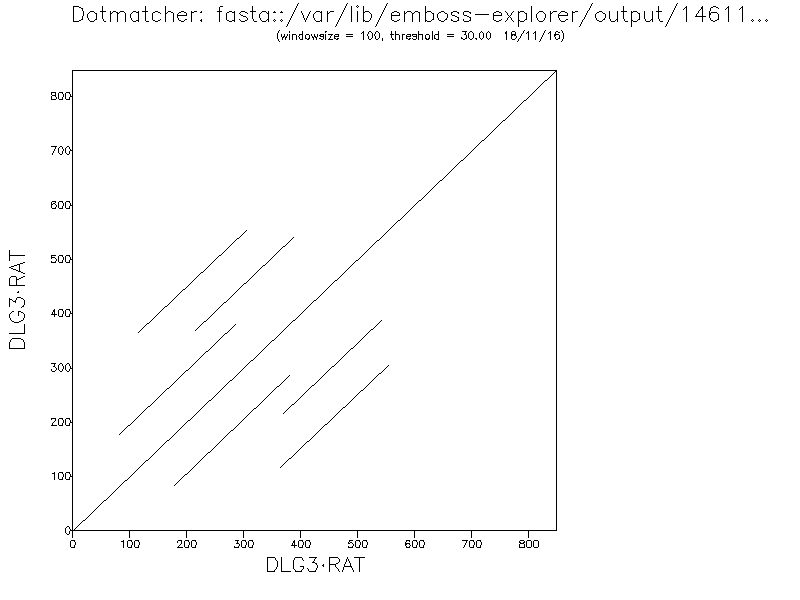
\includegraphics[width=\textwidth]{dotmatcher.png}
\caption{As seen on the picture, the \emph{three PDZ domains} are aligning to each other.
\href{http://www.bioinformatics.nl/emboss-explorer/output/146118/dotmatcher.1.png}{Source}}
\label{phytree1}
\end{figure}